\documentclass[xcolor={table}]{beamer}
\usetheme{Singapore}
\usepackage[utf8]{inputenc}
\usecolortheme{crane}
\usepackage{graphicx}
% \usepackage{iwona}
\usepackage{standalone}
\usepackage{tikz}
\usetikzlibrary{arrows}
\usetikzlibrary{decorations.markings}
\usetikzlibrary{calc}
\usetikzlibrary{shapes,snakes}
\usetikzlibrary{positioning,shapes.geometric}
\usepackage{amsmath}
\usepackage{amsfonts}
\usepackage{amsthm}
\usepackage{mathtools}
\usepackage{minted}
\usepackage{tcolorbox}
\usemintedstyle{trac}

\definecolor{lightblue}{RGB}{124,190,255}
\definecolor{darkgreen}{RGB}{24,145,0}
\definecolor{darkorange}{RGB}{220,110,0}
\definecolor{textorange}{HTML}{cc5200}
\definecolor{ciwyellow}{HTML}{fbbe28}
\definecolor{mplblue}{HTML}{1339cd}

\beamertemplatenavigationsymbolsempty
\setbeamerfont{caption}{size=\tiny}

\title{Open-Source Simulation with Ciw}
\author{Dr Geraint Palmer\\Supervisors: Prof Paul Harper \& Dr Vince Knight\\\textcolor{textorange}{www.geraintianpalmer.org.uk}\\\textcolor{textorange}{@GeraintPalmer} \vspace{-5mm}}
\date{Beale Lecture, February 2021}
\titlegraphic{
\includegraphics[width=2.5cm]{../cflogo.pdf}}

\begin{document}
\frame{\titlepage}

\begin{frame}
\begin{itemize}
  \item Reproducibility in simulation
  \item Detecting deadlock
  \item Extending Ciw
  \item Applications of Ciw
\end{itemize}
\end{frame}

\begin{frame}
\frametitle{Reproducibility}

\vfill

\begin{itemize}
  \item $R^1$: Re-runnable
  \item $R^2$: Repeatable
  \item $R^3$: Reproducible
  \item $R^4$: Reusable
\end{itemize}

\vfill

\scriptsize{\textcolor{textorange}{2018. \textit{Benureau, FCY., ac Rougier, NP.}. \textbf{Re-run, Repeat, Reproduce, Reuse, Replicate: Transforming Code into Scientific Contributions}. Frontiers in neuroinformatics.}}
\end{frame}


\begin{frame}
\scriptsize{\textcolor{textorange}{$\bullet$ 2013. \textit{Sandve, GK., et al.}, \textbf{Ten simple rules for reproducible computational research}. PLoS Comput Biol 9(10)}}\\
\scriptsize{\textcolor{textorange}{$\bullet$ 2014. \textit{Wilson, G., et al.}, \textbf{Best practices for scientific computing}. PLoS Biol 21(1)}}

\vspace{1mm}

\begin{columns}
\begin{column}{0.5\textwidth}
\large{
\begin{itemize}
  \item Automate!
  \item Readability
  \item Access
  \item Collaboration
  \item Testing
  \item Version control
\end{itemize}
}
\end{column}
\begin{column}{0.5\textwidth}
\onslide<2>{
\begin{tcolorbox}[colback=ciwyellow!20, colframe=ciwyellow, height=1.7cm, valign=center]
\centering
\LARGE{Readable}
\end{tcolorbox}
\begin{tcolorbox}[colback=mplblue!20, colframe=mplblue, height=1.7cm, valign=center]
\centering
\LARGE{Modular}
\end{tcolorbox}
\begin{tcolorbox}[colback=textorange!20, colframe=textorange, height=1.7cm, valign=center]
\centering
\LARGE{Extendible}
\end{tcolorbox}
}
\end{column}
\end{columns}

\vspace{2mm}

\onslide<2>{
\scriptsize{\textcolor{textorange}{2001. \textit{Kilgore, RA.}. \textbf{Open source simulation modeling language (sml)}. In Proceedings of the 33nd conference on Winter simulation (pp. 607–613).}}
}
\end{frame}


\begin{frame}

\begin{center}
\footnotesize{\textcolor{textorange}{https://ciw.readthedocs.io/}}\\
\footnotesize{\textcolor{textorange}{https://github.com/CiwPython/Ciw}}\\
\footnotesize{\textcolor{textorange}{\texttt{pip install ciw}}}
\end{center}

\begin{center}

\includegraphics[width=0.4\textwidth]{../images/ciwlogo}
\end{center}

\scriptsize{\textcolor{textorange}{2019. \textit{Palmer, GI., Knight, VA., Harper, PR., and Hawa, AL.}. \textbf{Ciw: An Open Source Discrete Event Simulation Library}. Journal of Simulation 13(1) (pp. 68-82).}}
\end{frame}

\begin{frame}
\begin{center}
\includestandalone[width=\textwidth]{../images/tandem_queues}
\end{center}
\end{frame}

\begin{frame}
\begin{center}
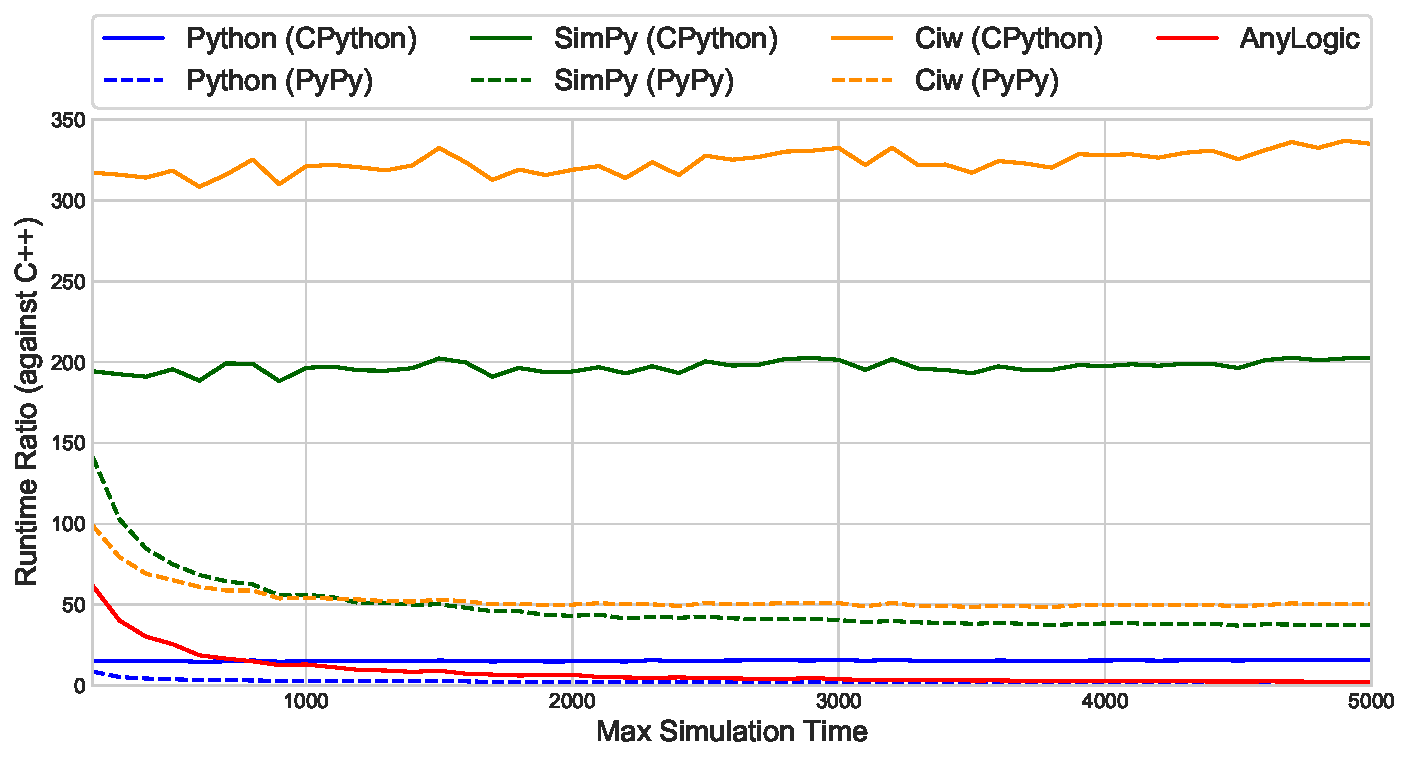
\includegraphics[width=0.8\textwidth]{../OR60/runtimes}
\end{center}
\end{frame}

\begin{frame}
\frametitle{Deadlock}
\begin{center}
\includestandalone[width=0.55\textwidth]{../images/gridlock}
\end{center}
\scriptsize{\textcolor{textorange}{2018. \textit{Palmer, GI., Harper, PR., and Knight, VA.}. \textbf{Modelling Deadlock in Open Restricted Queueing Networks}. European Journal of Operational Research 266(2) (pp. 609-621).}}
\end{frame}

\begin{frame}
\begin{center}
\centering
\includestandalone[width=0.5\textwidth]{../images/buildup}
\end{center}
\end{frame}

\begin{frame}
\begin{center}
\includestandalone[width=0.9\textwidth]{../images/buildupdigraph}
\end{center}
\end{frame}

\begin{frame}
    \frametitle{Times to Deadlock}
    \centering
    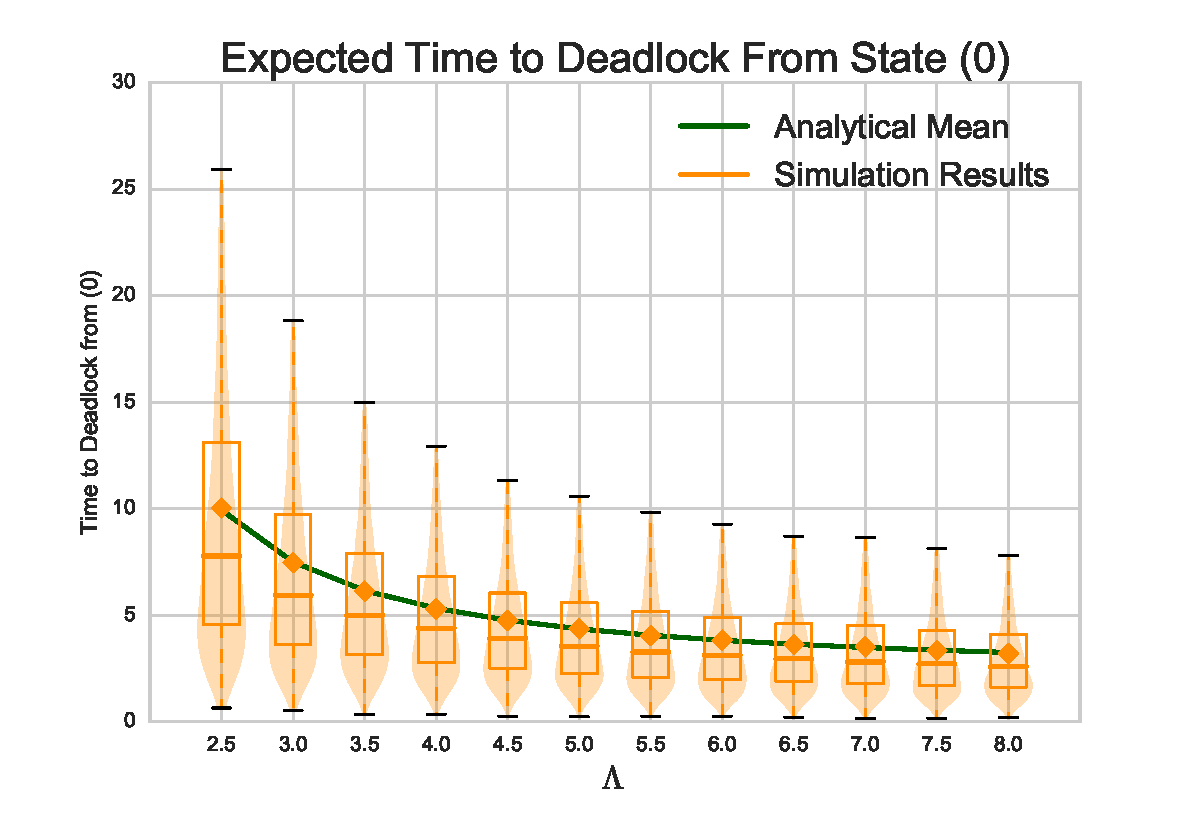
\includegraphics[width=0.45\textwidth]{../images/varyL_1Nms}
    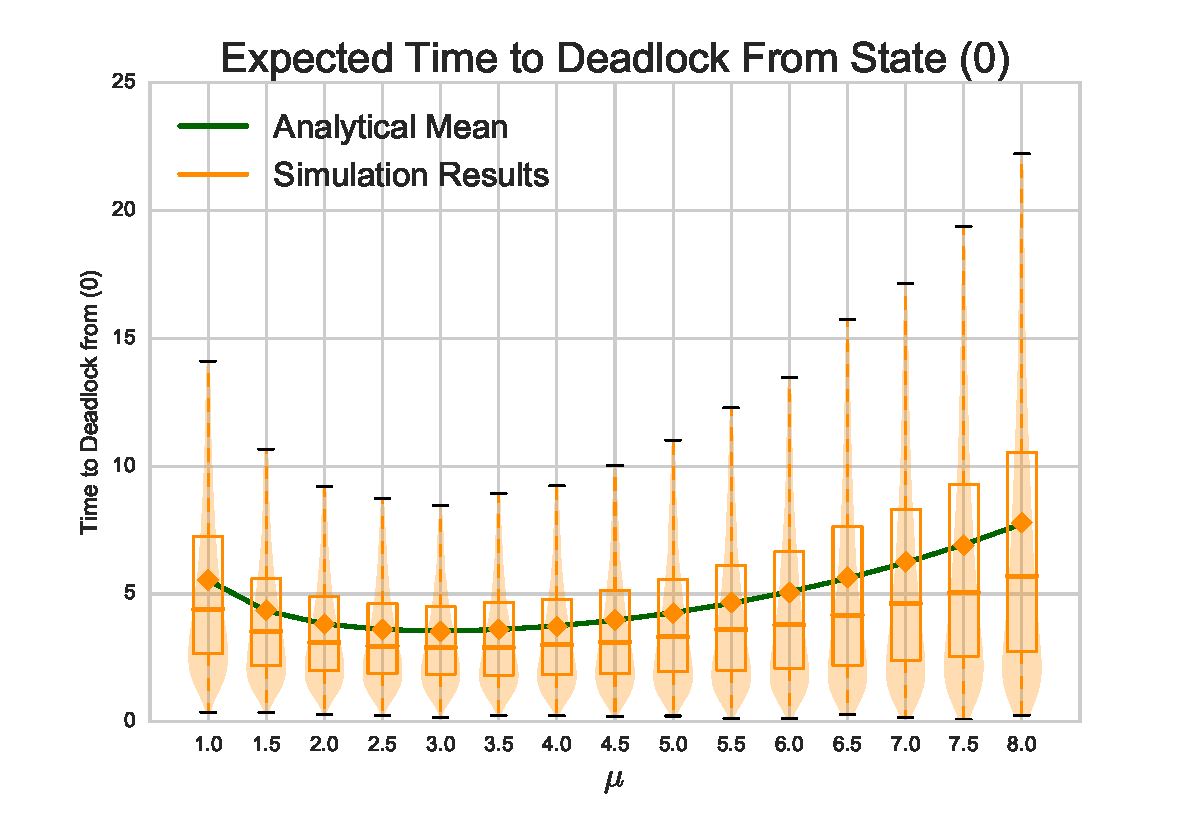
\includegraphics[width=0.45\textwidth]{../images/varymu_1Nms}\newline
    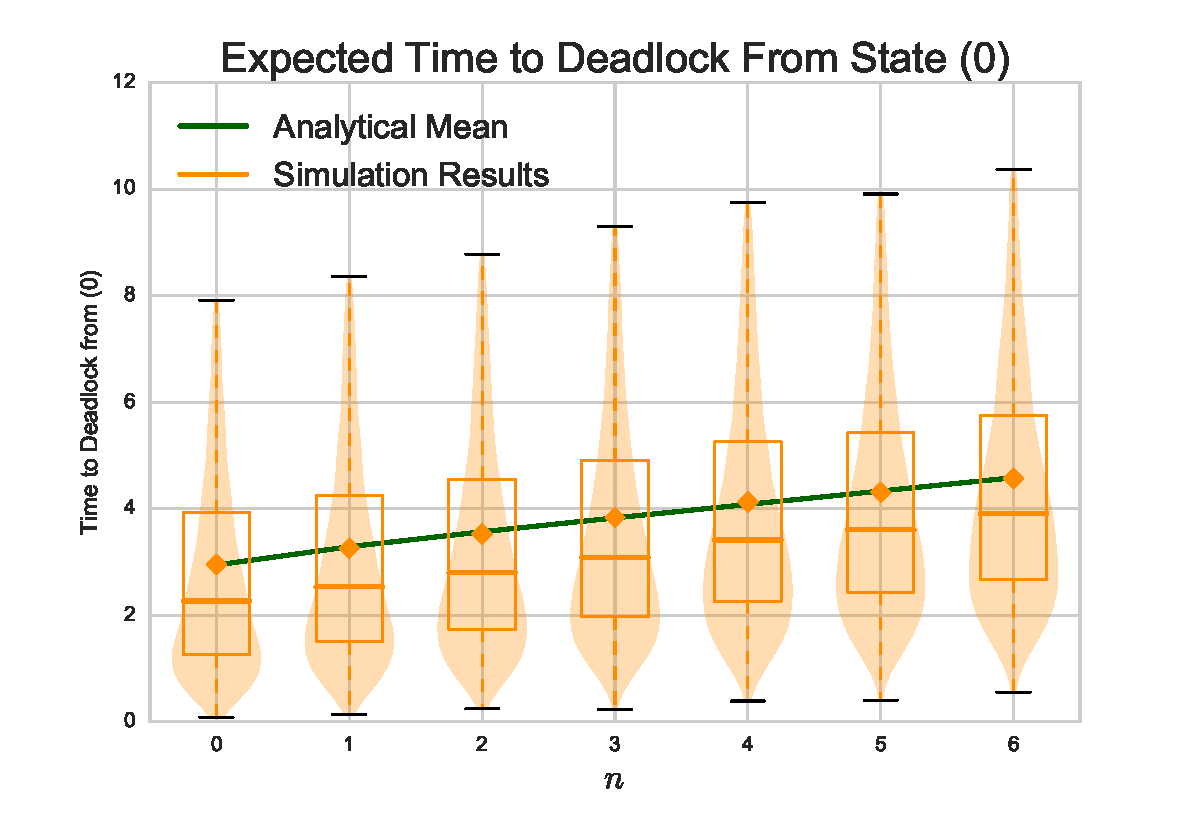
\includegraphics[width=0.45\textwidth]{../images/varyn_1Nms}
    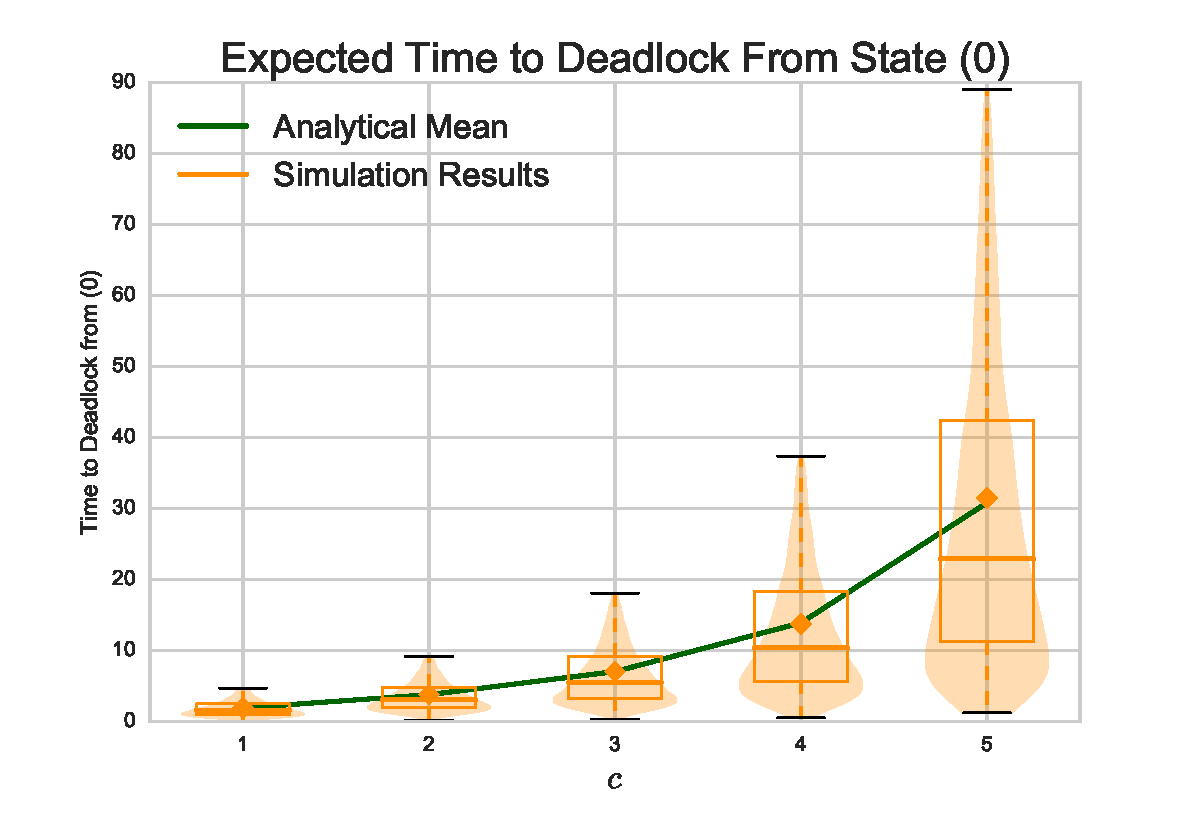
\includegraphics[width=0.45\textwidth]{../images/varyc_1Nms}
\end{frame}

\begin{frame}
\frametitle{Extendible}
\end{frame}

\begin{frame}
\begin{center}
\includestandalone[width=0.9\textwidth]{../images/hs-diagram}
\end{center}
\end{frame}

\begin{frame}
\begin{center}
\includestandalone[width=\textwidth]{../images/3phaseapprach}
\end{center}
\end{frame}

\begin{frame}
\frametitle{Applications of Ciw}
\begin{center}
\includestandalone[width=\textwidth]{../images/venn}
\end{center}
\end{frame}

\frame{\titlepage}

\end{document}
